\begin{figure}[htbp]\centering
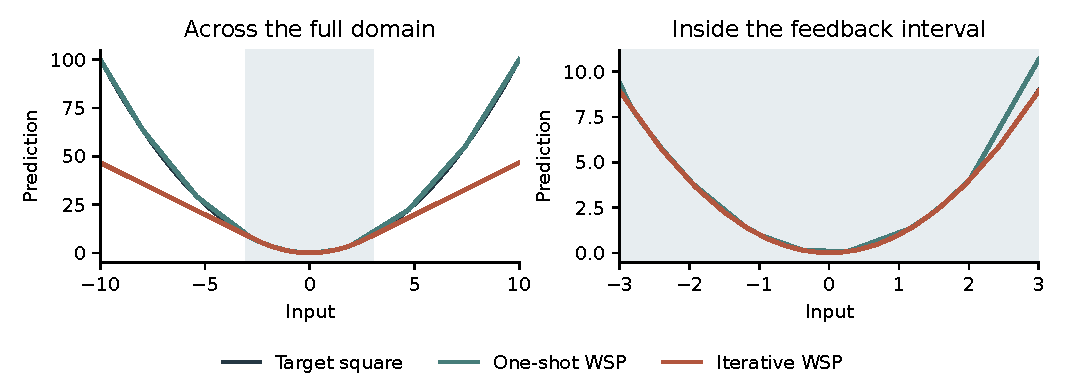
\includegraphics[width=\linewidth]{square_continuation.pdf}
\caption{The effect of central feedback on one square network with 16 hidden units and 50 coefficients. This examples-only run uses random start 164. The shaded interval supplied the training and development inputs. Iteration moved all changes of slope into that interval. At input 10, the selected revised network predicts 46.6765 against the target 100. The right panel shows the same functions restricted to the feedback interval.}\label{fig:square_continuation}
\end{figure}
